\section{The hybrid model}
\label{sec:CodeDocHybrid}

The hybrid model is the a model that is composed of both the electricity market model and the policy process model. These two models are connected with the goal of having policy agents influence what is going on in the electricity market. The policy agents will react to what is going on in the electricity market and will attempt to influence what is going on in the electricity market model. They will do so by implementing policy instruments that they perceive will help them reach their goals. These goals could be a decrease in emissions or an increase in international trade with France for example.

This chapter details the module interface that needs to be built to connects both models. This both considers the bridge that needs to be constructed to exchange data between the models and considers the specification of the policy process model which is now a generic model. This means specifying the problem tree and defining a set of policy instruments.

%%%%%%%%%%%%
\subsection{The hybrid model}
\label{ssec:hybridModel}

The hybrid model is presented in \autoref{fig:ModuleInterface-09}. The diagram outlines the two models and how information is transmitted from one to the other. The key performance indicators from the electricity market model are used to inform the truth agent which then relays the information to the active agents (policy makers and policy entrepreneurs) to inform their beliefs. At the end of the policy emergence model, if a policy instrument has been selected, it is transmitted to the electricity market model through a change in the exogenous parameters. This will then affect the system's outputs. This cycle goes on until the end of the simulation. Note that the electricity market model might be run for a period of a month to six months for every run of the policy process model.

\begin{figure}
\centering
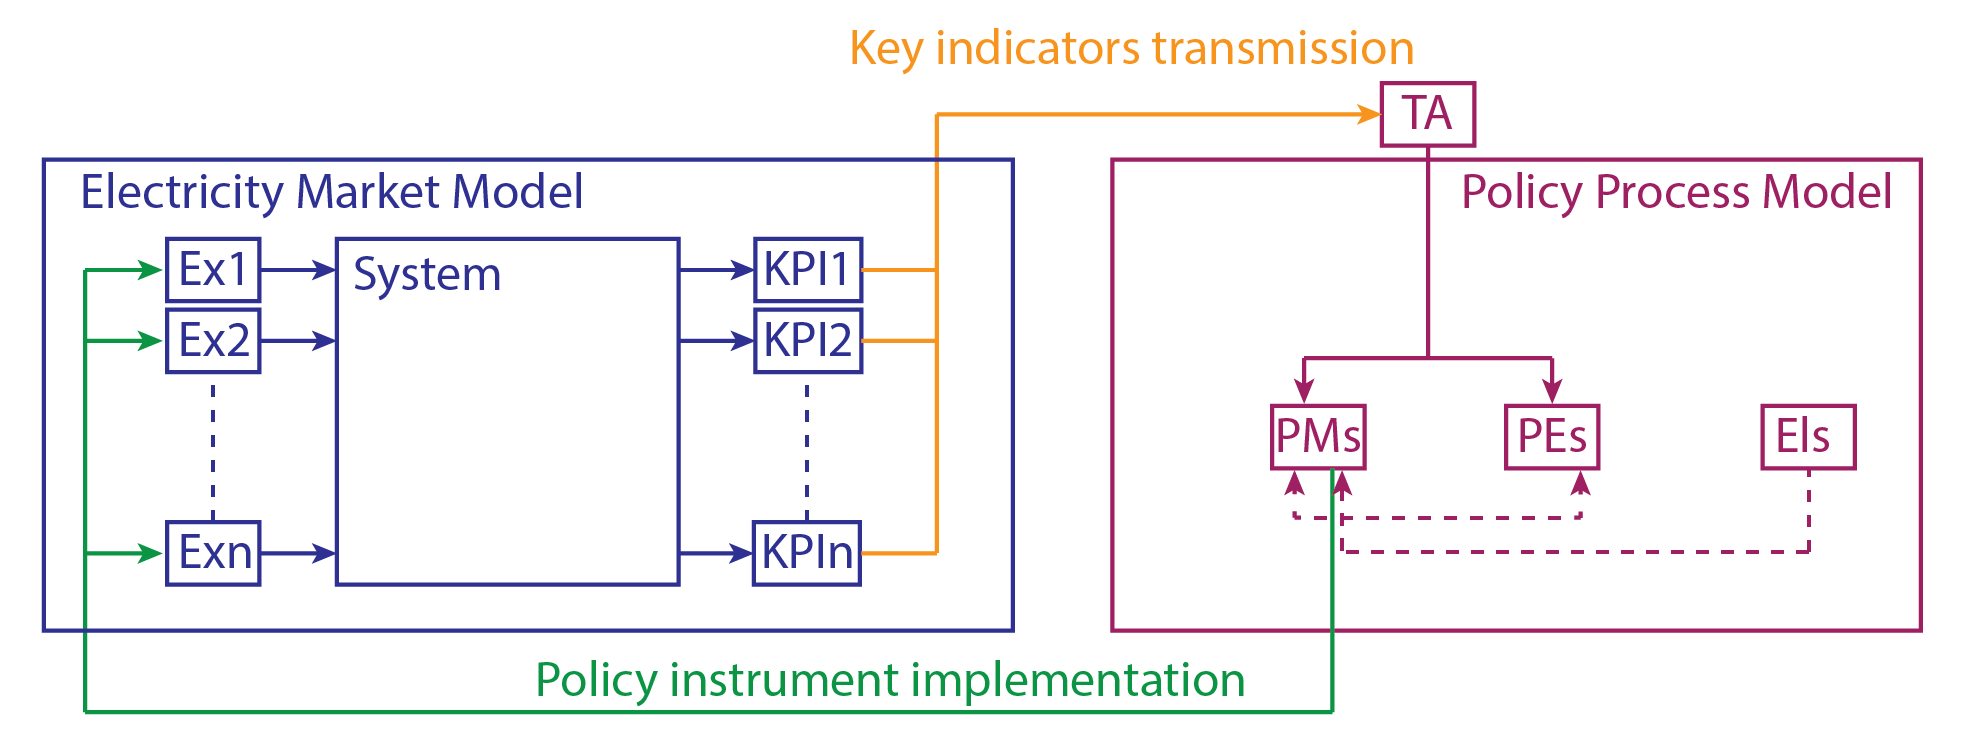
\includegraphics[width=\linewidth, keepaspectratio]{figures/ModuleInterface-09}
\caption{Diagram of the hybrid model.}
\label{fig:ModuleInterface-09}
\end{figure}

%%%%%%%%%%%% end of subsection

%%%%%%%%%%%%
\subsection{The problem tree}
\label{ssec:interfaceProblemTree}

To couple the models, the agents in the policy process need to be provided with a problem tree. This problem tree is specific to the electricity market model as it is informed by the key performance indicators from that model. This was highlighted in the previous section. Beyond this, the problems selected are also informed from previous work done by \cite{markard2016socio}. They identified a number of problems (they call these beliefs in their publication) that are specific to the Swiss context. These are however limited to the deep core and policy core levels. Secondary problems are not included or researched and are therefore taken from the model only.

The difficulty in the creation of the problem tree is to associate the right indicators to the right problems. The first step is to not consider the deep core problems. These are considered to be normative problems. They are beyond the boundaries of the model, out of the scope. They are not a crucial aspect of the process as it is focused on policy core problems so it does not make a big difference if deep core problems are considered or not. The next step is to consider the secondary problems. These can be found directly within the model. They are indicators that are made into secondary problems. Not all indicators are considered, only a few are selected. These are considered to be the important ones for the agents in the policy process. Finally, there is the selection of the policy core problems. These are, in general, aggregates of the secondary problems. They are calculated as a function of the main model indicators.

For the policy core problems, there is an additional aspect that needs to be considered. In work performed by \citeauthor{markard2016socio}, policy core problems within the Swiss electricity market subsystem were identified. These are: seriousness of the problem, role of the state, environment, economy and society. Several of these cannot be obtained from the model as they are outside of the boundaries of the model. However, the environment and economy can be considered. They are therefore selected as the policy core problems. \cite{markard2016socio} also identified four secondary problems. They are however not suitable for the model as they are more questions than problems. Furthermore, four secondary problems is not sufficient. It is for this reason that the secondary problems are only selected from the model. Ultimately, the policy core problems are calculated using linear equations that include a number of the indicators used for the secondary problems.

Overall, the problem tree is given as follows:

\begin{itemize}
\item Policy core problems:
	\begin{itemize}
	\item Economy
	\item Environment
	\end{itemize}
\item Secondary problems:
	\begin{itemize}
	\item Renewable energy production
	\item Electricity prices
	\item Renewable energy investments
	\item Domestic level emissions
	\item Imported emissions
	\end{itemize}
\end{itemize}

The economy takes into account elements related to profits of firms along with the security of supply of the country. The environment takes into account aspects such as the emissions, the amount of renewable energy and the amount of imported emissions.

%From markard2016socio, no deep core beliefs. Policy core beliefs are: seriousness of the problem, role of the state, environment, economy and society. In total, they identified 18 policy core beliefs. Most of these are beyond the scope of the model. The secondary beliefs identified are: phase out of nuclear, new nuclear plants, expansion of RES targets, expansion of energy demand targets, electricity suppliers role to fulfil efficiency targets.

%\begin{itemize}
%\item DC0 - Economy
%\item DC1 - Ecology
%\item PC0 - Security of supply
%\item PC1 - Profit levels - This is the average profits divided by the average revenues
%\item PC2 - Emissions - This is the average of domestic and imported emissions.
%\item S0 - Renewable energy production - This is calculated as the amount of renewable energy produced locally divided by the amount of energy produced overall.
%\item S1 - Nuclear production - This is the average production of nuclear over the total domestic production.
%\item S2 - Fossil fuel production - This is the average production of gas over the total domestic electricity production.
%\item S3 - Amount of imports
%\item S4 - Amount of exports - This is the average total amount of exports divided by the total demand
%\item S5 - Electricity prices - This is the price average. A maximum average price of 100 is assumed.
%\item S6 - Investment levels - This is the amount of investment (renovation + construction spent) over the amount of 
%\item S7 - Imported emission levels - This is the sum of all imported emissions from fossil fuel power plants divided by the total imported electricity. A maximum has to be found for normalisation based on average values.
%\end{itemize}

%%%%%%%%%%%% end of subsection

%%%%%%%%%%%%
\subsection{The policy instruments}
\label{ssec:interfaceInstruments}

The policy instruments within the policy tree are implemented using incremental increases and decreases in the following exogenous parameters.

\begin{enumerate}
\item Solar subsidies [+/- 0.02]
\item Wind turbine permit times [+/- 0.02]
\item Agent's hurdle rate  [+/- 0.01]
\item Carbon tax on fossil fuel imports [+/- 5]
\item Carbon tax on domestic fossil fuel [+/- 5]
\end{enumerate}

%%%%%%%%%%%% end of subsection